\documentclass[a4paper,11pt]{article}
\usepackage{a4wide}
\usepackage{fullpage}
\usepackage[utf8x]{inputenc}
\usepackage[toc,page]{appendix}
\usepackage[pdftex]{graphicx} % za slike
\usepackage{setspace}
\usepackage{color}
\definecolor{light-gray}{gray}{0.95}
\definecolor{mygray}{rgb}{0.5,0.5,0.5}
\usepackage{listings} % za vključevanje kode
\renewcommand{\baselinestretch}{1.2} % za boljšo berljivost večji razmak

\usepackage{bm}

\definecolor{vgray}{rgb}{0.408, 0.467, 0.639}
\usepackage[colorlinks, linkcolor={vgray}, citecolor={vgray}, urlcolor={vgray}]{hyperref}

\usepackage[font=small,labelfont=bf]{caption}	% for image side to table?


%
%		Python hylighting
%		Code from: http://tex.stackexchange.com/questions/83882/how-to-highlight-python-syntax-in-latex-listings-lstinputlistings-command
%
\usepackage{color}
\definecolor{deepblue}{rgb}{0,0,0.5}
\definecolor{deepred}{rgb}{0.6,0,0}
\definecolor{deepgreen}{rgb}{0,0.5,0}
\usepackage{listings}

\lstset{ % nastavitve za izpis kode, sem lahko tudi kaj dodaš/spremeniš
language=Python,
basicstyle=\footnotesize,
basicstyle=\ttfamily\footnotesize\setstretch{1},
backgroundcolor=\color{light-gray},
numberstyle=\scriptsize\color{mygray}\textit,
numbers=left,
title=\lstname,
title=\lstname   
}


% Python style for highlighting
\newcommand\pythonstyle{\lstset{
language=Python,
otherkeywords={self},             % Add keywords here
keywordstyle=\footnotesize\color{deepblue},
emph={MyClass,__init__},          % Custom highlighting
emphstyle=\footnotesize\color{deepred},    % Custom highlighting style
stringstyle=\color{deepgreen},
%frame=tb,                         % Any extra options here
showstringspaces=false            % 
}}

% Python environment
\lstnewenvironment{python}[1][]
{
\pythonstyle
\lstset{#1}
}
{}

% Python for external files
\newcommand\pythonexternal[2][]{{
\pythonstyle
\lstinputlisting[#1]{#2}}}

% Python for inline
\newcommand\pythoninline[1]{{\pythonstyle\lstinline!#1!}}

%
%		End code from web
%

\title{Seam Carving on PyOpenCL arhitecture}
\author{Niko Colnerič}
\date{\today}

\begin{document}

\maketitle

\begin{abstract}
The aim of this work is to test the ability of parallel computation architectures.
We first implement seam carving algorithm for content aware image resizing in pure Python.
Next, we implement the crucial parts of the algorithm in PyOpenCL.
Doing so, we are able to run it in parallel using either multiple CPU cores or on GPU.
The results show up to $53\times$~speed-up in both cases in comparison to single thread Python code.
\end{abstract}

\section{Introduction}
Seam carving \cite{Avidan2007} is an algorithm for content-aware image resizing.
In contrast to basic resizing techniques — like squeezing or cropping — it takes into account the content of the image and tries to resize it by removing its less important parts.
To define the importance image's region we employ some kind of energy function.
The goal of this function is to tell us how important is each pixel of the image.
One simple approach is to just take the discrete derivatives of the image like in Eq. \ref{eq1}.
This was used throughout the majority of the original paper and has shown to be successful so we also employed this energy function.

\begin{equation}
e_1(\bm{I}) = \left| \frac{\partial}{\partial x} \bm{I} \right| + \left| \frac{\partial}{\partial y} \bm{I} \right|
\label{eq1}
\end{equation}

Once the importance of pixels is defined, we resize the image to desired size by iteratively removing \emph{seams}.
Seam is an 8-connected path of pixels either from left to right (horizontal seam) or from top to bottom (vertical seam).
Examples of energy plot and a vertical seam are depicted in Fig. \ref{fig1}.
Seams are calculated with the dynamic programming approach in a top to bottom (and analogously left to right) manner.
For each pixel we sum its energy along with the minimal energy of the optimal path to the three pixels above (up, up-and-left, up-and-right).
When we traverse the whole image the last row contains the min-cost paths to each of the pixels in the last row.
We select the one with the minimal cost and then backtrack from its position to the top of the image to obtain a min-cost seam.

\begin{figure}[h!]
\begin{minipage}[b]{0.49\textwidth}

\includegraphics[width=\textwidth]{../img/nature_1024.png}
\end{minipage}
%\hfill
\begin{minipage}[b]{0.49\textwidth}
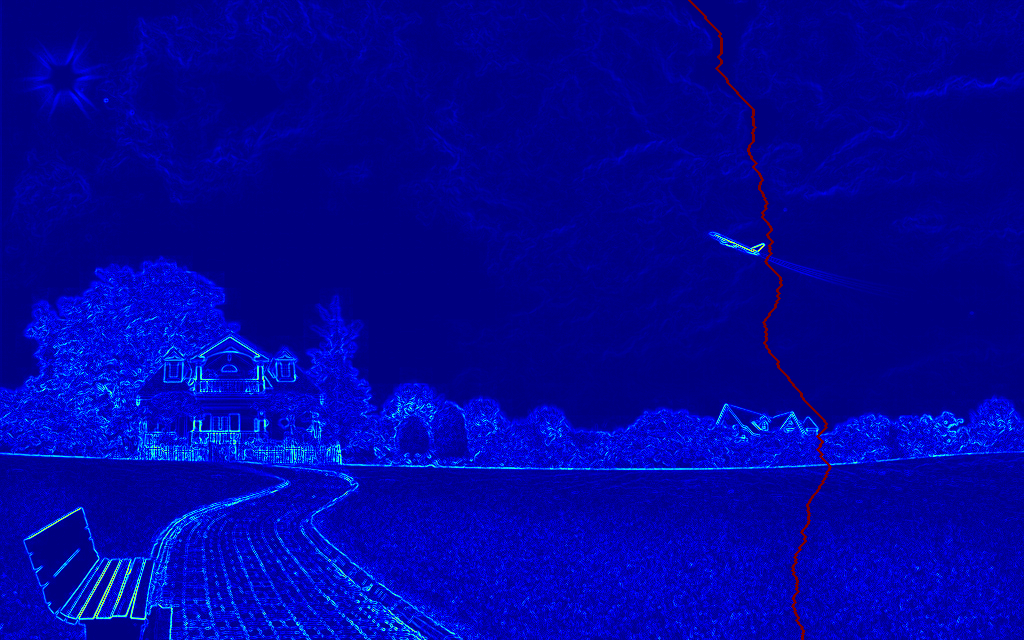
\includegraphics[width=\textwidth]{../results/energy-plot.png}
\end{minipage}
\captionof{figure}{Original image is shown on left. The right image presents the energy of the image, as defined in Eq. \ref{eq1}, along with one vertical seam in red color.}
\label{fig1}
\end{figure}

If we are only resizing in one dimension — either by height or width — we do this by iteratively finding one seam and removing it.
By repeating this $n$ times, we shrink the image by its height (width) by $n$ pixels.
However, when shrinking in both dimensions, the problem of optimal order arises.
Since our goal is to preserve as much \emph{energy} in the image as possible and different permutations of seam removal results in different loss of energy, we must find the optimal order.
Again, we employ a dynamic algorithm.
We initialize the transportation map $\bm{T}(0, 0) = 0$ and the first row/column with the cost of removing just horizontal/vertical seams.
$\bm{T}(i, j)$ will contain the optimal cost of removing $i$ horizontal and $j$ vertical seams.
We fill the transportation map $\bm{T}(i, j)$ by considering the best of two options: take $\bm{T}(i-1, j)$ and remove one vertical seam, or take $\bm{T}(i, j-1)$ and remove one horizontal seam.
Backtracking from $\bm{T}(n, m)$ gives the optimal order of seam removal for shrinking image's height by $n$ pixels and its width by $m$ pixels.

Note that seam carving can also be used for enlarging images, object removal, object amplification or constructing multi-size images.
However, we only focus on image shrinking by either one or both dimensions (along with the optimal order of seam removal).

\section{Implementation}
We first implemented seam carving in pure Python for shrinking the image's height and width along with the optimal order of seam removal.
All the source code is attached in appendix \ref{app-code} and also available online at \url{https://github.com/nikicc/seam-carving}.
Here we will only discuss the crucial parts that were also implemented in PyOpenCL — that is energy calculation and seam finding — and compare the single thread Python code to the PyOpenCL kernel code.

\subsection{Image's energy calculation}
To calculate the image's energy we used Eq. \ref{eq1}.
Since we processed color images, we sum the derivatives for each of the colors.
The crucial part of Python code, presented in Lst. \ref{code1}, is coming from the method \pythoninline{def get\_energy\_image(img)}.
We loop through each image's pixel, calculate the derivative and store it in the \pythoninline{energy[h, w]}.
Note that this code could be written much more efficiently using numpy on per-row basis rather than per-pixel basis.
We did not optimize it like this, to prevent numpy from automatically utilizing multiple cores for such calculations.

\pagebreak

\begin{figure}[h!]
\begin{python}[label=code1,caption=Python code for energy calculation.]
for h in range(height):
    for w in range(width):
        w_l = max(0, w-1)
        w_r = min(w+1, width-1)
        h_u = max(0, h-1)
        h_d = min(h+1, height-1)
        energy[h, w] = sum(abs(img[h_u, w, :] - img[h_d, w, :])) + \
                       sum(abs(img[h, w_l, :] - img[h, w_r, :]))
\end{python}
\end{figure}


Code from Lst. \ref{code1} was rewritten to OpenCL code shown on Lst. \ref{code2}.
Note that the $3D$ image array was first linearized and sent as a $1D$ array.
Therefore, we first need to translate the linear index back to $x$, $y$ and $z$ coordinates.
Later we also need the inverse mapping back to linear index which is provided as macro \pythoninline{LINEAR}.
In this kernel code we calculate the derivatives for each color separately and we sum them up for all colors afterwards in Python.

\begin{python}[label=code2,caption=OpenCl kernel code for energy calculation.]
#define MIN(X, Y) (((X) < (Y)) ? (X) : (Y))
#define MAX(X, Y) (((X) > (Y)) ? (X) : (Y))
#define ABS(x) ((x)<0 ? -(x) : (x))
#define LINEAR(h, w, d, H, W, D) (h*(W*D) + w*(D) + d)

__kernel void energy(__global float* img, __global float* res,
                     int H, int W, int D)
{
    // get liner index
    int index = get_global_id(0);

    // convert index to 3D coordinates
    int d = index % D;
    int h = index / (W*D);
    int w = (index / D) % W;

    // sanity check
    /*
    int back = LINEAR(h, w, d, H, W, D);
    if(back==index){
        res[index] = -42;
    }
    */

    // "border safe" indices
    int wl = MAX(0, w-1);
    int wr = MIN(w+1, W-1);
    int hu = MAX(0, h-1);
    int hd = MIN(h+1, H-1);

    // derivative value
    float der = 0;

    // left-right
    int bl = LINEAR(h, wl, d, H, W, D);
    int br = LINEAR(h, wr, d, H, W, D);
    der += ABS(img[bl] - img[br]);


    // up-down
    int bu = LINEAR(hu, w, d, H, W, D);
    int bd = LINEAR(hd, w, d, H, W, D);
    der += ABS(img[bu] - img[bd]);

    res[index] = der;
}
\end{python}

\subsection{Finding optimal seams}
Once we fill the \pythoninline{energy} matrix, we can use it to find optimal min-cost seams.
Python version of this is presented in Lst. \ref{code3} and comes from method \pythoninline{def find_seam_vertical(energy)}.
We use array \pythoninline{M} to store costs of optimal paths to each of the pixels and \pythoninline{backtrace} for backtracking the min-cost seam.

\begin{python}[label=code3,caption=Python code for finding vertical seams. Code for horizontal seams is analogous.]
for h in range(1, height):
    for w in range(width):
        w_l = max(0, w-1)
        w_r = min(w+2, width)

        ind, val = min_argmin(M[h-1, w_l:w_r])
        M[h, w] = energy[h, w] + val
        backtrace[h, w] += ind - 1
\end{python}

The code from Lst. \ref{code3} was rewritten to OpenCL kernel code presented in Lst. \ref{code4}.
We calculate this on per-row basis, meaning that we sent one row for execution to OpenCL.
Then get back results and execute the next row.
This could be implemented much more efficiently using synchronization methods.

\begin{python}[label=code4,caption=OpenCl kernel code for finding optimal seams.]
__kernel void find_seam(__global float* m, __global float* energy,
                        __global float* new_m, __global float* back, int W)
{
    // get index
    int w = get_global_id(0);

    // "border safe" indices
    int wl = MAX(0, w-1);
    int wr = MIN(w+1, W-1);

    // enlarge the path by one
    float val = INFINITY;
    int ind;
    for(int i = 0; (i+wl) <= wr; i = i+1){
        if(m[i + wl] < val){
            val = m[i + wl];
            ind = i;
        }
    }

    // store energy
    new_m[w] = energy[w] + val;


    // store backtrack pointers
    // special case for first element, since there is no "left"
    if(w == 0){
        ind += 1;
    }
    back[w] = ind-1;
}
\end{python}


\section{Results}
We presents the time measurements of out Python and PyOpenCL implementations.
All following results are obtained on a series of one image in different sizes — from $32\times20$ up to $1024\times640$ pixels.
Experiment were run on a computer containing Intel Core i7 processor ($4$ cores, $8$ threads) and Intel Iris Pro integrated GPU.
We measured the total time to remove $25$ vertical seams and we report on the average times per seam.
Fig. \ref{fig:times} shows total times for removing a seam, Fig. \ref{fig:energy} and Fig. \ref{fig:seam} show the times for calculating energy and finding a seam respectively.
All plots are in logarithmic scale.
We also show exact times per seam in Tab. \ref{tab:times}.


\begin{figure}[h!]
\begin{minipage}[b]{0.49\textwidth}
	\centering
	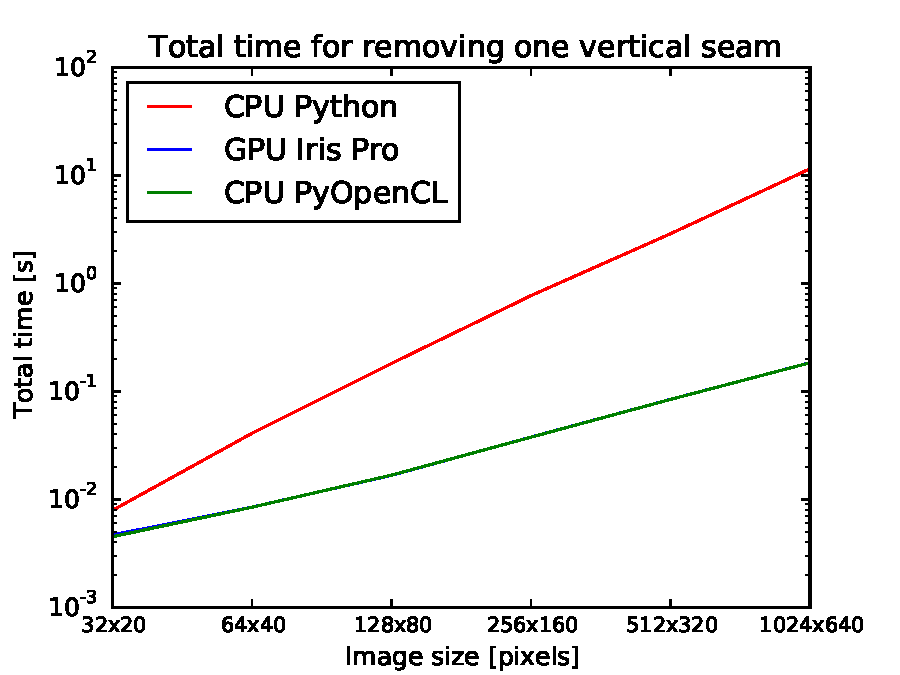
\includegraphics[width=\textwidth]{../results/total-time.pdf}
	\captionof{figure}{Total times for removing one seam.}
	\label{fig:times}
\end{minipage}
\hfill
\begin{minipage}[b]{0.47\textwidth}
	\centering
	\begin{footnotesize}
	\begin{tabular}{cccc}
	\hline	
	Size     			& Python 				& PyOpenCL 	& Speedup 	\\
	$[$pixels$]$		&	[s]					&	CPU [s]				&					\\ \hline
	32x20    		& $\;\ 0.007$		& $0.004$     	& $1$      	\\
	64x40    		& $\;\ 0.035$		& $0.010$      & $3$      	\\
	128x80   		& $\;\ 0.155$		& $0.021$      & $7$      	\\
	256x160  	& $\;\ 0.695$		& $0.043$      & $16$      	\\
	512x320  	& $\;\ 2.727$		& $0.093$      & $29$      	\\
	1024x640 	& $10.243$		& $0.191$      & $53$      	\\ \hline
	\end{tabular}
	\end{footnotesize}
	\captionof{table}{Total times for removing one vertical seam on CPU with pure Python vs. PyOpenCL.}
	\label{tab:times}
\end{minipage}
\end{figure}


\begin{figure}[h!]
\begin{minipage}[b]{0.48\linewidth}
\centering
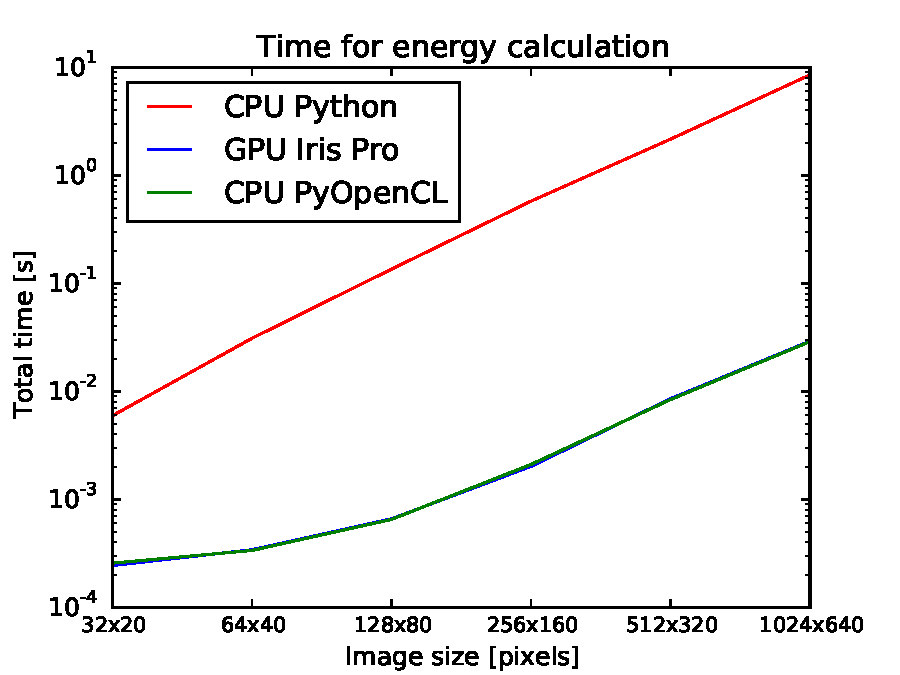
\includegraphics[width=\textwidth]{../results/energy-time.pdf}
\captionof{figure}{Times for calculating image's energy.}
\label{fig:energy}
\end{minipage}
\hfill
\begin{minipage}[b]{0.48\linewidth}
\centering
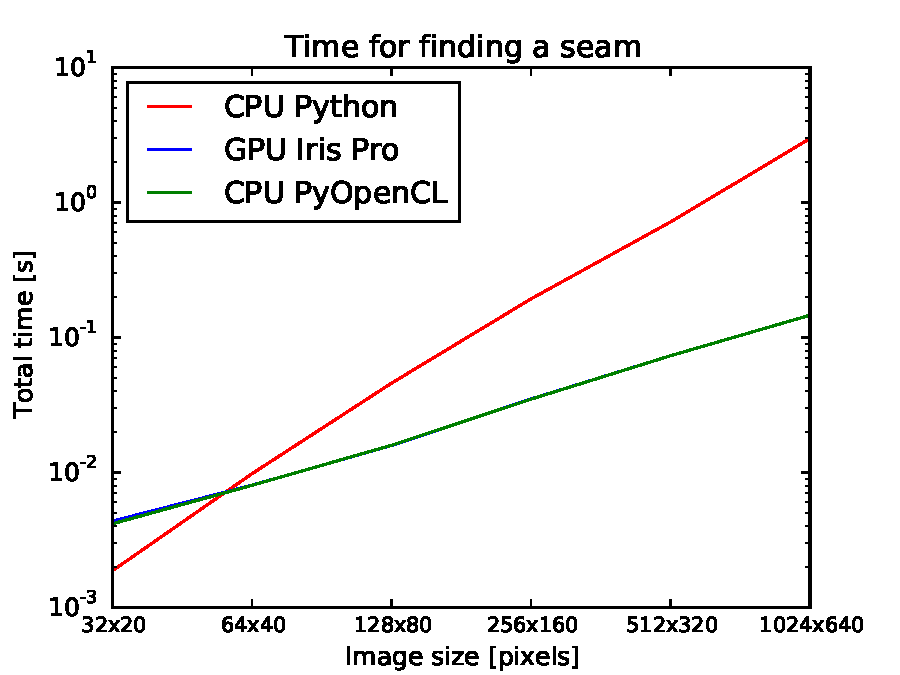
\includegraphics[width=\textwidth]{../results/seam-time.pdf}
\captionof{figure}{Times for finding one vertical seam.}
\label{fig:seam}
\end{minipage}
\end{figure}

Using PyOpenCL we were able to significantly speedup out algorithm — even up to $53\times$ for image with size $1024\times640$.
The time for removing one seam was brought down from $~10s$ to $~0.2$s.
Interestingly, running PyOpenCL implementation all $8$ CPU threads requires almost exactly the same time as running it on integrated GPU.
Most importantly, Fig. \ref{fig:times} shows that the time spent grows more slowly with PyOpenCL that pure Python implementations, which is indicated by a smaller slope.


\section{Usage}
Fig. \ref{fig:scenario} shows one source image re-targeted to different sizes.
We show images shank by $100px$ in height, width, and height $\&$ width.
Image is more suitable for shrinking by width, due to the sky.
When shrinking by height, we introduce noticeable irregularities since sky pixels on same height have different colors. Note that important parts — house, bench, pavement and trees — remain more or less the same on all images. The majority of reduction in done in the sky and grass and is therefore almost unnoticeable, especially when only reducing the width.

\begin{figure}[h!]
\begin{minipage}[b]{0.48\linewidth}
\setlength\fboxsep{5pt}
\setlength\fboxrule{0pt}
\centering
\fbox{
\includegraphics[width=\textwidth]{../img/nature_1024.png}}
\fbox{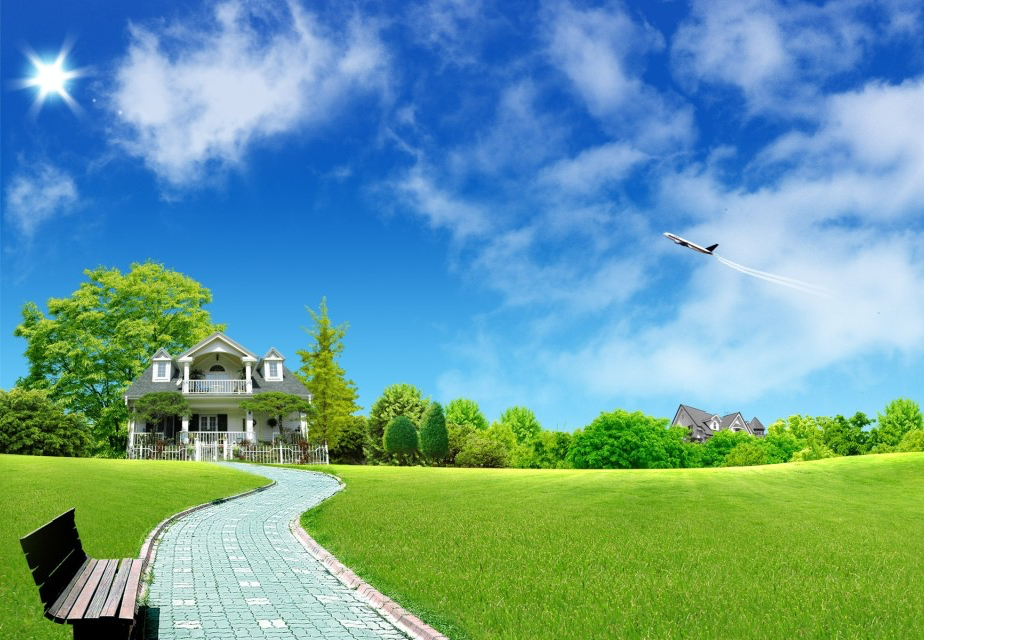
\includegraphics[width=\textwidth]{../results/nature_1024-100w-0h.png}}

\end{minipage}
\hfill
\begin{minipage}[b]{0.48\linewidth}

\centering
\setlength\fboxsep{5pt}
\setlength\fboxrule{0pt}
\fbox{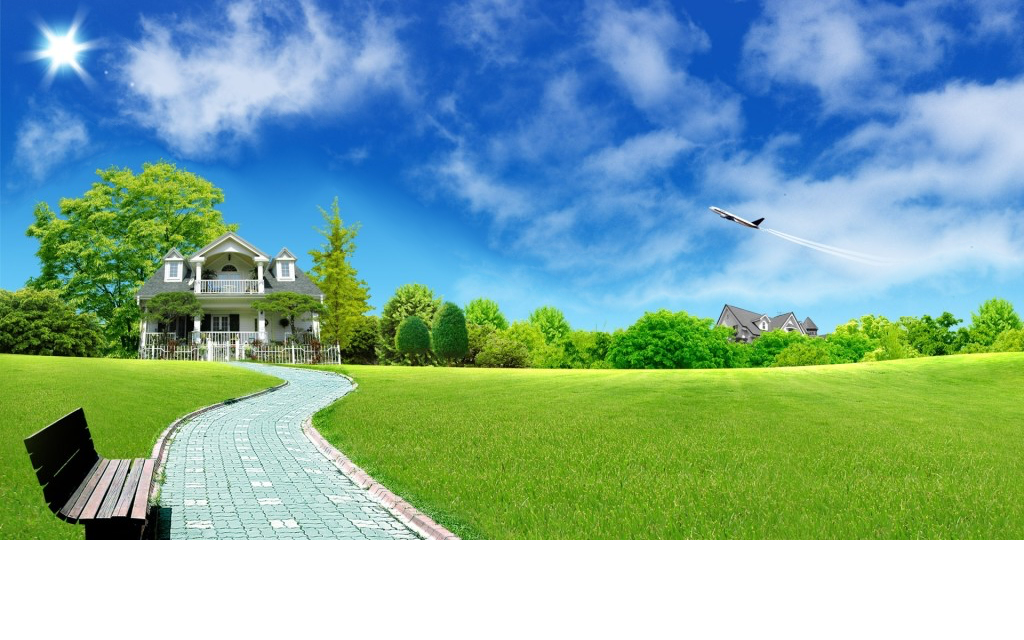
\includegraphics[width=\textwidth]{../results/nature_1024-0w-100h.png}}
\fbox{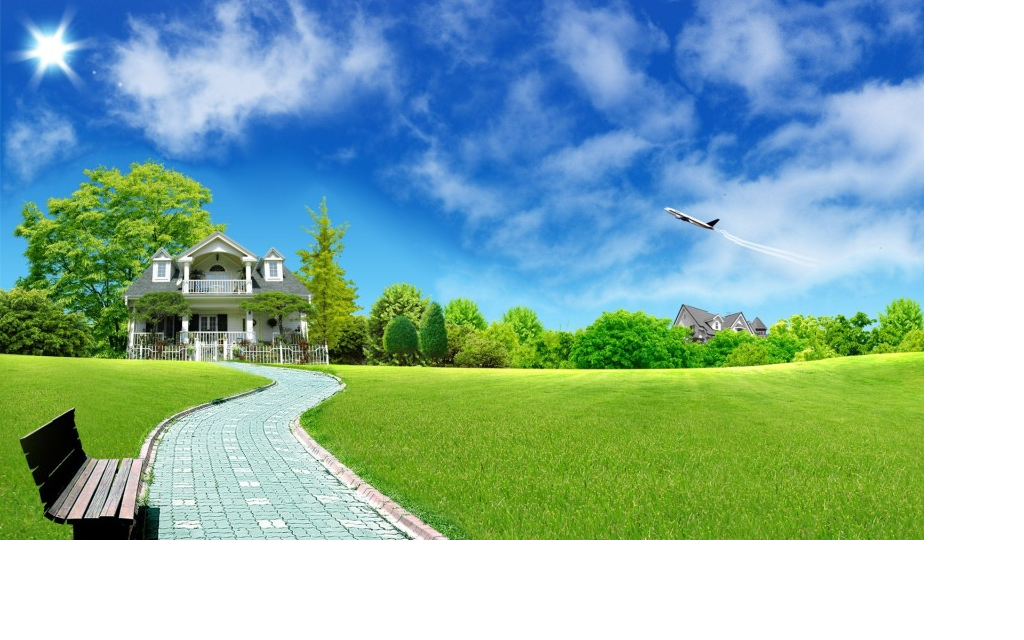
\includegraphics[width=\textwidth]{../results/nature_1024-100w-100h.png}}

\end{minipage}
\captionof{figure}{Original image ($1024px\times 640px$) is shown on top left position. Top right is shrank by height for $100px$. Bottom left is shrank by width for $100px$. Bottom right is shrank by height and width, each for $100px$.}
\label{fig:scenario}
\end{figure}


\section{Conclusion}
We implemented seam carving algorithm first in pure Python and then also in PyOpenCL.
The beauty of PyOpenCL implementation is that it can be run on heterogeneous systems; that is, out code can be run either on CPU or GPU.
Our main goal was to test whether we can speed-up seam carving algorithm on parallel architectures.
Results have shown that using either multiple CPU cores or using GPU we are able to achieve significant speed-ups, even up to $53\times$.
Note, however, that the GPU we were using — Intel Iris Pro — is and integrated one and not a dedicated one.
We presume the speed-up could be even larger on a capable dedicated GPU.

\bibliographystyle{acm}
\bibliography{references} 

\appendix
\appendixpage

\section{\label{app-code}Source code}
We list here all the source code.
File \emph{get\_energy.cl} contains the OpenCL kernel code, file \emph{seamcarve.py} contains the pure Python code along with the PyOpenCL code that calls \emph{get\_energy.cl}.
All this code is also available online at \url{https://github.com/nikicc/seam-carving}.

\pythonexternal{../get_energy.cl}
 
\pythonexternal{../seamcarve.py}

\end{document}
